% Drawing 72/03-1 -- folder 72, batch 03, archive page 46 (PDF page 47).
% Transcription: dans la marge gauche, un petit segment gradué « $i \geqslant 2$, $i-1$, $i$ », deux arcs joignant les points voisins
% Kind: graduated segment with arcs. Method 2 (schematic redraw from the facsimile). Status: ok.
% Notes: In the margin: "i >= 2", a horizontal segment, a dot at i-1, a short thick stroke and a tick, i at the right; two arcs below joining neighbouring points. The label above i-1 reads only as an i on the crop; i-1 after the transcription.
% Coordinates: 1 unit = 1 mm = 1/100 of the crop width (bbox in page fractions: [0.14, 0.235, 0.33, 0.275]).
% Redrawn by Claude (claude-opus-5-5), issue #73, 2026-11-07; not checked by a human; not compiled (no TeX in the session).
% Rights: reproduces part of the work -- behind RENDER_TRANSCRIPTS, never published by itself.
\documentclass[tikz,border=3pt]{standalone}
\usepackage{amsmath,amssymb}
\usetikzlibrary{patterns,arrows.meta}
\tikzset{pencil/.style={black!45}, struck/.style={black!35}, mark/.style={circle,draw,inner sep=1.3pt}, pt/.style={circle,fill,inner sep=0.9pt}, opt/.style={circle,draw,fill=white,inner sep=1.1pt}}
\begin{document}
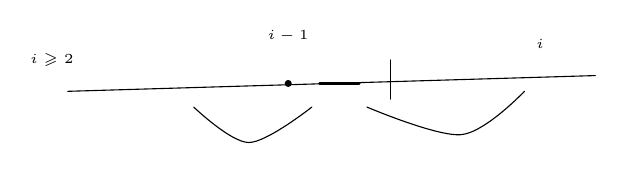
\begin{tikzpicture}[x=1mm,y=1mm,line cap=round,line join=round,font=\scriptsize]
\node[inner sep=1pt] at (8,-9) {\tiny $i\geqslant 2$};
\draw (10,-13) -- (77,-11);
\node[pt] at (38,-12) {};
\draw[very thick] (42,-12) -- (47,-12);
\draw (51,-9) -- (51,-14);
\draw plot[smooth, tension=0.55] coordinates {(26,-15) (33,-19.5) (41,-15)};
\draw plot[smooth, tension=0.55] coordinates {(48,-15) (60,-18.5) (68,-13)};
\node[inner sep=1pt] at (38,-6) {\tiny $i-1$};
\node[inner sep=1pt] at (70,-7) {\tiny $i$};
\end{tikzpicture}
\end{document}
